\documentclass[aspectratio=169,xcolor={dvipsnames}]{beamer}

% XeLaTeX packages
\usepackage{fontspec}
\usepackage{xcolor}
\usepackage{tikz}
\usetikzlibrary{positioning}
\usepackage{booktabs}
\usepackage{amsmath}
\usepackage{amsthm}
\usepackage{caption}
\usepackage{graphicx}
\usepackage{listings}
\usepackage{biblatex}

% Bibliography
\addbibresource{references_new.bib}

% Modern theme configuration
\usetheme{Boadilla}
\usecolortheme{default}

% Define complementary palette based on VU Blue
\definecolor{VUBlue}{HTML}{0057B7}
\definecolor{Endeavour}{HTML}{0754AA}
\definecolor{AbsoluteZero}{HTML}{055AB9}
\definecolor{ScienceBlue}{HTML}{0360C8}
\definecolor{RustyNail}{HTML}{8E4F09}
\definecolor{RichGold}{HTML}{9C5608}
\definecolor{LightGray}{HTML}{E8E9EA}
\definecolor{Charcoal}{HTML}{222831}

% Set theme colors
\setbeamercolor{frametitle}{bg=VUBlue, fg=white}
\setbeamercolor{title}{fg=VUBlue}
\setbeamercolor{structure}{fg=ScienceBlue}
\setbeamercolor{alerted text}{fg=RustyNail}
\setbeamercolor{block title}{bg=AbsoluteZero, fg=white}
\setbeamercolor{block body}{bg=LightGray, fg=Charcoal}
\setbeamercolor{alertblock title}{bg=RustyNail, fg=white}
\setbeamercolor{alertblock body}{bg=LightGray, fg=Charcoal}

% Font settings
\setmainfont{Liberation Sans}
\setsansfont{Liberation Sans}
\setmonofont{Liberation Mono}[Scale=0.9]

% Custom commands
\newcommand{\highlight}[1]{\textcolor{RustyNail}{\textbf{#1}}}
\newcommand{\code}[1]{\texttt{\small #1}}
\newcommand{\phase}[1]{\textcolor{ScienceBlue}{\textbf{Phase #1}}}

% Configure listings
\lstset{
  basicstyle=\ttfamily\footnotesize,
  backgroundcolor=\color{LightGray},
  frame=single,
  breaklines=true
}

% Title page info
\title{Privacy-Preserving Synthetic Trajectory Generation}
\subtitle{An Integrated DiffTraj-LM-TAD Framework for Taxi Route Anomaly Detection}
\author{Mateusz Kędzia}
\institute{MSc Artificial Intelligence \\ Vrije Universiteit Amsterdam}
\date{Thesis Progress Presentation -- July 2025}

% Custom title page
\defbeamertemplate*{title page}{customized}[1][]
{%
  \vbox{}
  \vfill
  \begingroup
    \centering
    \begin{beamercolorbox}[sep=8pt,center,#1]{title}
      \usebeamerfont{title}\inserttitle\par%
      \ifx\insertsubtitle\@empty%
      \else%
        \vskip0.25em%
        {\usebeamerfont{subtitle}\usebeamercolor[fg]{subtitle}\insertsubtitle\par}%
      \fi%     
    \end{beamercolorbox}%
    \vskip1em\par
    \begin{beamercolorbox}[sep=8pt,center,#1]{author}
      \usebeamerfont{author}\insertauthor
    \end{beamercolorbox}
    \begin{beamercolorbox}[sep=8pt,center,#1]{institute}
      \usebeamerfont{institute}\insertinstitute
    \end{beamercolorbox}
    \begin{beamercolorbox}[sep=8pt,center,#1]{date}
      \usebeamerfont{date}\insertdate
    \end{beamercolorbox}\vskip0.5em
  \endgroup
  \vfill
}

\begin{document}

% --- Title Slide ---
\begin{frame}[plain]
  \vspace{1.5cm}
  \centering
  {\usebeamerfont{title}\color{VUBlue}\Huge\textbf{Privacy-Preserving Synthetic Trajectory Generation}}
  
  \vspace{0.5em}
  {\usebeamerfont{subtitle}\color{RichGold}\Large An Integrated DiffTraj-LM-TAD Framework}
  
  \vspace{1.5em}
  {\usebeamerfont{author}\large Mateusz Kędzia}
  
  \vspace{0.5em}
  {\usebeamerfont{institute}\normalsize MSc Artificial Intelligence \\ Vrije Universiteit Amsterdam}
  
  \vspace{1em}
  {\usebeamerfont{date}\small Thesis Progress Presentation -- July 2025}
\end{frame}

% --- Section: Introduction ---
\section{Introduction}

\begin{frame}{The Core Challenge}
  \begin{block}{}
    \centering
    \Large \textbf{Privacy vs. Utility Paradox}
    
    \vspace{1em}
    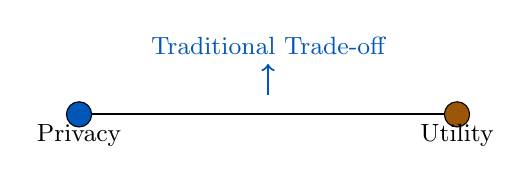
\begin{tikzpicture}[scale=0.8]
      % Privacy vs Utility scale
      \draw[thick] (0,0) -- (6,0);
      \draw[fill=VUBlue] (0,0) circle (0.2);
      \draw[fill=RichGold] (6,0) circle (0.2);
      \node[below, font=\small] at (0,0) {Privacy};
      \node[below, font=\small] at (6,0) {Utility};
      \draw[thick,->,VUBlue] (3,0.3) -- (3,0.8);
      \node[above,VUBlue, font=\small] at (3,0.8) {Traditional Trade-off};
    \end{tikzpicture}
    
    \vspace{1em}
    \textcolor{Charcoal}{\small Standard privacy methods degrade spatio-temporal patterns}
  \end{block}
\end{frame}

\begin{frame}{Key Problems}
  \begin{block}{}
    \begin{itemize}
      \item \highlight{Data Scarcity}: Limited access to real trajectory datasets
      \item \highlight{Privacy Barriers}: Sensitive location information blocks research
      \item \highlight{Detection Limitations}: Need preserved patterns for anomaly detection
    \end{itemize}
  \end{block}
\end{frame}

\begin{frame}{Our Innovation}
  \begin{alertblock}{}
    \centering
    \Large \textbf{Privacy by Design} \\
    \vspace{0.5em}
    $+$ \\
    \vspace{0.5em}
    \textbf{High Utility} \\
    \vspace{0.5em}
    $+$ \\
    \vspace{0.5em}
    \textbf{Anomaly Detection Ready}
  \end{alertblock}
\end{frame}

% --- Section: Methodology ---
\section{Methodology}

\begin{frame}{Framework Overview}
  \begin{block}{}
    \centering
    \Large \textbf{3-Phase Bootstrap Framework}
  \end{block}
  
  \vspace{1em}
  \begin{center}
    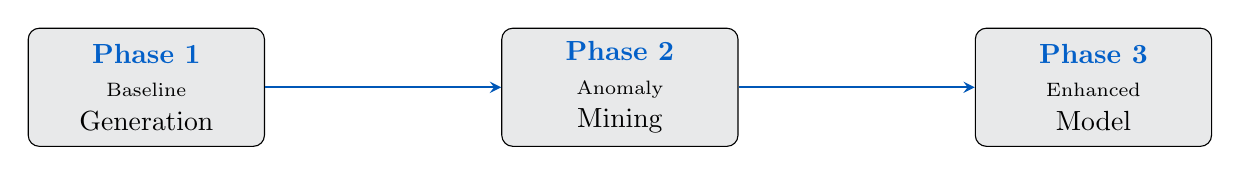
\begin{tikzpicture}[node distance=3cm, every node/.style={align=center}]
      % Nodes
      \node[draw, fill=LightGray, rounded corners, minimum width=3cm, minimum height=1.5cm] (phase1) {\textbf{\phase{1}}\\\scriptsize Baseline\\Generation};
      \node[draw, fill=LightGray, rounded corners, right=of phase1, minimum width=3cm, minimum height=1.5cm] (phase2) {\textbf{\phase{2}}\\\scriptsize Anomaly\\Mining};
      \node[draw, fill=LightGray, rounded corners, right=of phase2, minimum width=3cm, minimum height=1.5cm] (phase3) {\textbf{\phase{3}}\\\scriptsize Enhanced\\Model};
      % Arrows
      \draw[thick, VUBlue,->, >=stealth] (phase1) -- (phase2);
      \draw[thick, VUBlue,->, >=stealth] (phase2) -- (phase3);
    \end{tikzpicture}
  \end{center}
  
  \vspace{1em}
  \begin{block}{}
    \centering
    \textit{``Bootstraps anomaly generation without pre-labeled dataset''}
  \end{block}
\end{frame}

\begin{frame}{Key Innovation: Bootstrap Approach}
  \begin{block}{Why This Works}
    \begin{itemize}
      \item \textbf{Iterative Learning}: Each cycle improves understanding
      \item \textbf{Controlled Generation}: Rule-based curation
      \item \textbf{Privacy First}: From distributions, not copies
    \end{itemize}
  \end{block}
\end{frame}

% --- Section: Core Models ---
\section{Core Models}

\begin{frame}{DiffTraj: Diffusion-Based Generation}
  \begin{block}{}
    \centering
    \Large \textbf{White Noise} $\rightarrow$ \textbf{Reverse Denoising} $\rightarrow$ \textbf{Realistic Trajectory}
    
    \vspace{0.5em}
    \small \cite{zhuDiffTrajGeneratingGPS2023}
  \end{block}
  
  \vspace{1em}
  \begin{columns}[T,onlytextwidth]
    \begin{column}{0.48\textwidth}
      \begin{block}{Architecture}
        \begin{itemize}
          \item 1D-CNN residual network
          \item Attention mechanisms
          \item GPS coordinate compatible
        \end{itemize}
      \end{block}
    \end{column}
    \hspace{0.04\textwidth}
    \begin{column}{0.48\textwidth}
      \begin{block}{Advantages}
        \begin{itemize}
          \item Training stability
          \item High-fidelity samples
          \item Inherent privacy protection
        \end{itemize}
      \end{block}
    \end{column}
  \end{columns}
\end{frame}

\begin{frame}{LM-TAD: Language Model for Trajectories}
  \begin{block}{}
    \centering
    \Large \textbf{GPS Trajectory} $\rightarrow$ \textbf{Token Sequence} $\rightarrow$ \textbf{Perplexity Score}
    
    \vspace{0.5em}
    \small \cite{mbuyaTrajectoryAnomalyDetection2024}
  \end{block}
  
  \vspace{1em}
  \begin{columns}[T,onlytextwidth]
    \begin{column}{0.48\textwidth}
      \begin{block}{Process}
        \begin{itemize}
          \item Autoregressive prediction
          \item Transformer architecture
          \item Interpretable scoring
        \end{itemize}
      \end{block}
    \end{column}
    \hspace{0.04\textwidth}
    \begin{column}{0.48\textwidth}
      \begin{block}{Perfect for Bootstrap}
        \begin{itemize}
          \item No labeled data required
          \item Online detection capability
          \item Clear anomaly explanations
        \end{itemize}
      \end{block}
    \end{column}
  \end{columns}
\end{frame}

% --- Section: Privacy Framework ---
\section{Privacy Framework}

\begin{frame}{Three-Layer Defense}
  \begin{center}
    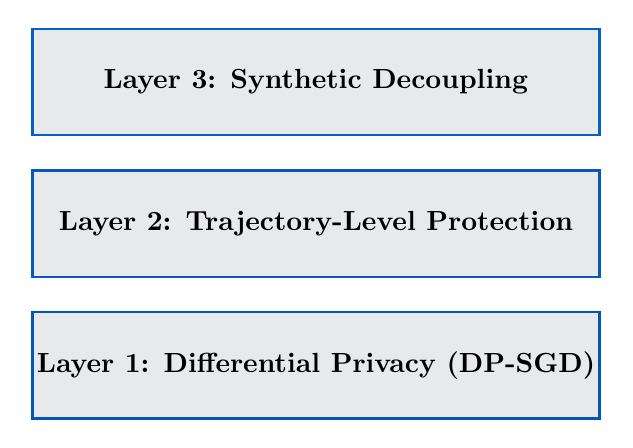
\begin{tikzpicture}[scale=0.9]
      % Layer 1
      \draw[fill=LightGray, draw=VUBlue, thick] (0,0) rectangle (8,1.5);
      \node at (4,0.75) {\textbf{Layer 1: Differential Privacy (DP-SGD)}};
      
      % Layer 2
      \draw[fill=LightGray, draw=AbsoluteZero, thick] (0,2) rectangle (8,3.5);
      \node at (4,2.75) {\textbf{Layer 2: Trajectory-Level Protection}};
      
      % Layer 3
      \draw[fill=LightGray, draw=ScienceBlue, thick] (0,4) rectangle (8,5.5);
      \node at (4,4.75) {\textbf{Layer 3: Synthetic Decoupling}};
    \end{tikzpicture}
  \end{center}
  
  \vspace{1em}
  \begin{alertblock}{}
    \centering
    \textit{``Traditional privacy methods destroy spatio-temporal relationships''}
  \end{alertblock}
\end{frame}

\begin{frame}{Differential Privacy Integration}
  \begin{columns}[T,onlytextwidth]
    \begin{column}{0.48\textwidth}
      \begin{block}{DP-SGD Parameters}
        \begin{itemize}
          \item \textbf{Phase 1}: $\varepsilon = 2.0$
          \item \textbf{Phase 2}: $\varepsilon = 1.0$
          \item \textbf{Phase 3}: $\varepsilon = 0.5$
        \end{itemize}
      \end{block}
    \end{column}
    \hspace{0.04\textwidth}
    \begin{column}{0.48\textwidth}
      \begin{block}{Protection}
        \begin{itemize}
          \item Bounded influence
          \item Membership inference prevention
          \item Noise addition during training
        \end{itemize}
      \end{block}
    \end{column}
  \end{columns}
\end{frame}

% --- Section: Implementation Phases ---
\section{Implementation}

\begin{frame}{Phase 1: Baseline Generation}
  \begin{block}{}
    \centering
    \Large \textbf{Real Normal Data} $\rightarrow$ \textbf{Train DiffTraj} $\rightarrow$ \textbf{Synthetic Normal}
  \end{block}
  
  \vspace{1em}
  \begin{block}{Smart Filtering}
    \begin{itemize}
      \item \textbf{Duration}: Within $2\sigma$ of O-D medians
      \item \textbf{Distance}: $\leq 1.5 \times$ shortest path
      \item \textbf{Temporal}: Typical patterns only
    \end{itemize}
  \end{block}
\end{frame}

\begin{frame}{Phase 2: Anomaly Mining}
  \begin{block}{}
    \centering
    \Large \textbf{Synthetic Normal} $\rightarrow$ \textbf{LM-TAD} $\rightarrow$ \textbf{Labeled Anomalies}
  \end{block}
  
  \vspace{1em}
  \begin{columns}[T,onlytextwidth]
    \begin{column}{0.48\textwidth}
      \begin{block}{LM-TAD Scoring}
        \begin{itemize}
          \item Perplexity calculation
          \item Higher = more anomalous
          \item Interpretable results
        \end{itemize}
      \end{block}
    \end{column}
    \hspace{0.04\textwidth}
    \begin{column}{0.48\textwidth}
      \begin{block}{Rule-Based Curation}
        \begin{itemize}
          \item Route deviation rules
          \item Temporal delay detection
          \item Kinematic constraints
        \end{itemize}
      \end{block}
    \end{column}
  \end{columns}
\end{frame}

\begin{frame}{Phase 3: Iterative Refinement}
  \begin{block}{}
    \centering
    \Large \textbf{Normal + Anomalies} $\rightarrow$ \textbf{Retrain DiffTraj} $\rightarrow$ \textbf{Enhanced Model}
  \end{block}
  
  \vspace{1em}
  \begin{block}{Process Components}
    \begin{itemize}
      \item \textbf{Enriched Training}: 5-10\% anomalies
      \item \textbf{Iterative Cycles}: Generate $\rightarrow$ Mine $\rightarrow$ Refine
      \item \textbf{Conditional Generation}: Context-aware synthesis
    \end{itemize}
  \end{block}
\end{frame}

% --- Section: Evaluation ---
\section{Evaluation}

\begin{frame}{Experimental Design}
  \begin{block}{Cross-City Validation}
    \begin{table}[h]
      \centering
      \begin{tabular}{lll}
        \toprule
        \textbf{Dataset} & \textbf{Role} & \textbf{Purpose} \\
        \midrule
        \textbf{Beijing} & Primary & Framework development \\
        \textbf{Chengdu} & Validation & Cross-city generalization \\
        \textbf{Xi'an} & Validation & Urban diversity testing \\
        \bottomrule
      \end{tabular}
    \end{table}
  \end{block}
\end{frame}

\begin{frame}{Evaluation Metrics}
  \begin{columns}[T,onlytextwidth]
    \begin{column}{0.32\textwidth}
      \begin{block}{Detection Performance}
        \begin{itemize}
          \item Precision
          \item Recall
          \item F1-Score
          \item AUC-PR
        \end{itemize}
      \end{block}
    \end{column}
    \hspace{0.02\textwidth}
    \begin{column}{0.32\textwidth}
      \begin{block}{Data Quality}
        \begin{itemize}
          \item Resemblance
          \item Utility
          \item Privacy
          \item SDMetrics
        \end{itemize}
      \end{block}
    \end{column}
    \hspace{0.02\textwidth}
    \begin{column}{0.32\textwidth}
      \begin{block}{Privacy Protection}
        \begin{itemize}
          \item Membership inference
          \item Reconstruction attacks
          \item Privacy budgets
        \end{itemize}
      \end{block}
    \end{column}
  \end{columns}
\end{frame}

% --- Section: Contributions ---
\section{Contributions}

\begin{frame}{Key Contributions}
  \begin{block}{Technical Innovations}
    \begin{enumerate}
      \item \textbf{Integrated Framework}: First DiffTraj + LM-TAD combination
      \item \textbf{Bootstrap Methodology}: Anomaly generation without labels
      \item \textbf{Multi-Layer Privacy}: Comprehensive protection strategy
    \end{enumerate}
  \end{block}
  
  \vspace{1em}
  \begin{block}{Research Impact}
    \begin{itemize}
      \item Novel privacy-preserving trajectory research
      \item Reproducible evaluation framework
      \item Open-source implementation
    \end{itemize}
  \end{block}
\end{frame}

\begin{frame}{Project Timeline}
  \begin{block}{Implementation Progress}
    \begin{itemize}
      \item \phase{1}: \textcolor{AbsoluteZero}{\textbf{In Progress}} (baseline DiffTraj)
      \item \phase{2}: \textbf{Planned} (LM-TAD integration)
      \item \phase{3}: \textbf{Planned} (iterative refinement)
    \end{itemize}
  \end{block}
  
  \vspace{1em}
  \begin{block}{Next Steps}
    \begin{enumerate}
      \item Complete Phase 1 baseline
      \item Implement LM-TAD integration
      \item Develop rule-based curation
      \item Cross-city validation
    \end{enumerate}
  \end{block}
\end{frame}

\begin{frame}{Expected Outcomes}
  \begin{block}{Deliverables}
    \begin{itemize}
      \item \textbf{Synthetic Datasets}: Privacy-preserving anomaly data
      \item \textbf{Open Framework}: Reproducible research pipeline
      \item \textbf{Evaluation Results}: Comprehensive performance analysis
      \item \textbf{Research Publication}: Novel methodology contribution
    \end{itemize}
  \end{block}
\end{frame}

\begin{frame}[plain]
  \centering
  \Huge \textbf{Thank You}
  
  \vspace{0.5em}
  \Large \textbf{Questions \& Discussion}
  
  \vspace{1em}
  \begin{columns}[T,onlytextwidth]
    \begin{column}{0.48\textwidth}
      \begin{block}{Key Takeaways}
        \begin{itemize}
          \item \textbf{Privacy-Preserving}: Multi-layer protection
          \item \textbf{Bootstrap Approach}: No labeled data required
        \end{itemize}
      \end{block}
    \end{column}
    \hspace{0.04\textwidth}
    \begin{column}{0.48\textwidth}
      \begin{block}{}
        \begin{itemize}
          \item \textbf{Practical Framework}: Real-world applications
          \item \textbf{Open Research}: Reproducible and extensible
        \end{itemize}
      \end{block}
    \end{column}
  \end{columns}
\end{frame}

\begin{frame}[allowframebreaks]{References}
  \begin{block}{}
    \small
    \printbibliography[heading=none]
  \end{block}
\end{frame}

\end{document} 